\chapter{二元调制多符号条件归零接收机}
在上一章,我们系统讨论了高阶调制QAM信号的接收方案,
至此,常见的调制方案都已被比较系统的研究。
在这些方案中,通常都是针对单个符号设计的接收方案,
而正如第二章所述,采用针对编码后的多个符号设计的联合检测方案才有可能
逼近Holevo容量。因此这一章我们来讨论最简单的三种
调制方案的一种联合检测方案——条件归零接收机。


\section{MPPM信号条件归零接收机}
首先,我们来考虑一种特殊的编码方案,多脉冲脉冲位置调制(MPPM)信号。
与PPM信号的思想一样,信息被调制在脉冲的位置上面,
具有很高的能量效率,这在深空通信中具有潜在的应用价值\cite{hemmati2006deep}。
与PPM信号不同的是,它的每一个符号通常采用两个或者两个以上的脉冲
来加载信息。采用这种方式,
可以在保证的较高能量效率的同时,
还能有效的克服PPM信号低频谱效率的缺点\cite{sugiyama1989mppm}。
这在深空通信如地月通信、卫星到卫星通信等场景
具有潜在的优势\cite{hemmati2006deep,waseda2011numerical}。

\subsection{MPPM信号标准量子极限}
首先,我们先来从数学上定义MPPM信号符号集合。
设每一个MPPM信号符号有$M$个时隙,对每一个符号,
都有$L$个时隙有脉冲,而其他$M-L$个时隙没有脉冲,
我们称这种MPPM信号为L-M-PPM信号,如图\ref{fig:MPPM-DD}(\textit{a})所示。
一般的,我们只考虑$L \ge 2$的情形,$L=1$时就退化为单脉冲PPM的情形。
容易知道,这样的L-M-PPM信号的符号集合个数为
\begin{equation}
\binom{M}{L} = \frac{M(M-1)\cdots(M-L+1)}{L!}.
\end{equation}
例如当$M=4, L=2$时,2-4-PPM信号有$\binom{4}{2}=6$个,如果用1代表
有脉冲,而用0代表没有脉冲,那么这些信号可以编码为二进制码字
$\bm{c} = (c_1, c_2, \cdots, c_M)$,对2-4-PPM信号这6个码字为
\begin{equation}
\begin{array}{cccc}
1 & 0 & 0 & 1 \\
1 & 0 & 1 & 0 \\
1 & 1 & 0 & 0 \\
0 & 1 & 0 & 1 \\
0 & 1 & 1 & 0 \\
0 & 0 & 1 & 1   
\end{array}
\end{equation}
在将这些码字映射到量子态时,我们用相干态$\ket{0}$和$\ket{\alpha}$
分别代表0和1,用直积态
\begin{equation}
\ket{\gamma_1}\otimes\ket{\gamma_2}\otimes\cdots\otimes\ket{\gamma_M}, \\
\ket{\gamma_i} = \begin{cases}
                    \ket{0}, & c_i=0, \\
                    \ket{\alpha}, & c_i=1
                \end{cases}
\end{equation}
来表示每一个码字对应的信号。

\begin{figure}
\centering
  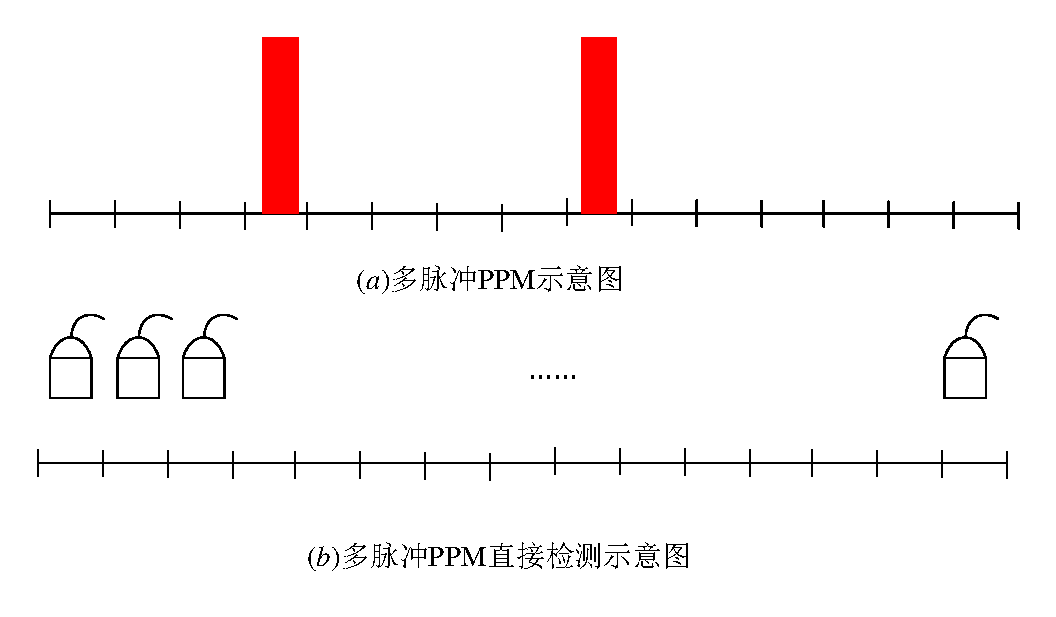
\includegraphics[width=0.8\textwidth]{figures/chap4/MPPM-DD}
  \caption{MPPM信号和直接检测示意图}
  \label{fig:MPPM-DD}
\end{figure}

在经典的光通信系统中,与PPM信号一样,采用直接检测的方法
对MPPM信号进行探测\cite{simon2003multi}。
直接检测探测方法利用一个ON-OFF探测器,
对每一个时隙进行独立的探测。
设每一个时隙的输出为$o_i$,如果有脉冲
$o_i=1$,否则$o_i=0$。
那么$M$个时隙对应的$M$个输出
构成输出序列$\bm{o} = (o_1,o_2,\cdots,o_M)$。
当所有的$M$个时隙都探测完毕,
然后通过最大似然准则进行译码判决\cite{simon2003multi}。
如果所有码字的先验概率是相同的(通信中通常都满足),这种判决准则使得平均错误概率最低。
对于给定的码字$\bm{c}_i$,输出序列为$\bm{o}$的条件概率为
\begin{equation}
\Pr{\bm{o} | \bm{c}_i} = \prod_{k=1}^M \left(1 - e^{-c_{ik}n} \right)^{o_{k}} \left(e^{-c_{ik}n} \right)^{1-o_{k}} .
\end{equation}
其中$\bm{c}_i=(c_{i1},\cdots,c_{iM})$
和$\bm{o}=(o_{1},\cdots,o_{M})$
分别为码字和输出序列,
$n=|\alpha|^2$是一个脉冲的平均光子数。
最大似然准则通过计算对给定的输出序列$\bm{o}$
每一个符号对应的条件概率,
选择出条件概率最大的符号进行判决,
该条件概率也称似然函数。

理想情况下,实际检测到脉冲数目$K \le L$,此时上述
条件概率也即是似然函数变为
\begin{equation}
\Lambda_i = \Pr{\bm{o} | \bm{c}_i} = \begin{cases} 
                                        \left(1 - e^{-n} \right)^{K} \left(e^{-n} \right)^{L-K}, & o_k \le c_{ik} \forall k,\\
                                        0,                                                       & \text{otherwise}.
                                    \end{cases}
\end{equation}
对于给定的码符号集合,$L$是相同的,
所以根据最大似然准则,对给定的输出序列$\bm{o}$,
只要满足$o_k \le c_{ik} \forall k$的码字对应的
似然函数是相同的。此时随机选择一个判决输出。
因此,对给定的码字$\bm{c}_i$,
在探测到$K$个光子时接收机正确探测的概率为
\begin{equation}
\Pr{\bm{c}_i | \bm{c}_i} = \frac{1}{\binom{M-K}{L-K}} \binom{L}{K} \left(1 - e^{-n} \right)^{K} \left(e^{-n} \right)^{L-K}.
\end{equation}
所以,这种检测方案的平均错误概率为
\begin{equation}
\begin{split}
P_e &= \frac{1}{\binom{M}{L}}\sum_{i=1}^{\binom{M}{L}} \sum_{K=0}^{L} \Pr{\bm{c}_i | \bm{c}_i, K}  \\
    &= \sum_{K=0}^{L} \frac{1}{\binom{M-K}{L-K}} \binom{L}{K} \left(1 - e^{-n} \right)^{K} \left(e^{-n} \right)^{L-K}.
\end{split}
\end{equation}
下面我们考虑大信号近似,即当$n \gg 1$时,可以忽略少检测到的脉冲数目大于1个的情况的概率,
即
\begin{equation}
\begin{split}
\Pr{\bm{c}_i | \bm{c}_i} &\approx (1-e^{-n})^L + \frac{L}{M-L+1} (1-e^{-n})^{L-1} e^{-n} \\
                            &\approx 1 - L\left(1 - \frac{1}{M-L+1} \right)e^{-n}.
\end{split}
\end{equation}
因此,这种检测方案的渐近性能为
\begin{equation}
\begin{split}
P_e & \approx L\left(1 - \frac{1}{M-L+1} \right)e^{-n} \\
    & = L\left(1 - \frac{1}{M-L+1} \right)e^{-|\alpha|^2}.
\end{split}
\end{equation}



\subsection{MPPM信号Helstrom极限}
一般而言,MPPM信号并不具有几何均匀对称性,
为了求得这种信号的最优量子检测的性能,
需要如QAM信号那样求解半正定规划问题\ref{eq:Hel-SDP}。
因此,我们需要得到密度矩阵。
与QAM信号不同的是,MPPM信号是直积态,
如果采用QAM信号那种将每一个时隙的信号在Fork态中展开,
然后截取长度为$l$的向量,那么要表达整个直积态信号,
所需要的向量维度为$l^M$,将随着时隙数目$M$指数增长,
这将为计算带来困难。
所以这里我们采用Smit正交化的方法\cite{lzw2010LA,zyh2007szjsff},
构造一组新的基向量$\ket{e_i}$。
为方便计,我们用矢量$\ket{\psi_i}$表示这$N = \binom{M}{L}$个直积态信号,
那么基向量$\ket{e_i}$可以表达为
\begin{equation}
\begin{split}
\ket{u_1} &= \ket{\psi_1}, \ket{e_1} = \frac{\ket{u_1}}{\sqrt{\bra{u_1}\ket{u_1}}}\\
\ket{u_2} &= \ket{\psi_2} - \bra{e_1}\ket{\psi_2}\ket{e_1}, \ket{e_2} = \frac{\ket{u_2}}{\sqrt{\bra{u_2}\ket{u_2}}}\\
          &\qquad\qquad \vdots \\
\ket{u_N} &= \ket{\psi_N} - \sum_{k=1}^{N-1} \bra{e_k}\ket{\psi_N}\ket{e_k}, \ket{e_k} = \frac{\ket{u_N}}{\sqrt{\bra{u_N}\ket{u_N}}}.
\end{split}
\end{equation}
设在该基向量上,$\ket{\psi_i} =\bm{c}_i = (c_{i1} \quad c_{i2} \dots c_{in})^T$,
那么有
\begin{equation}
\begin{split}
c_{11} &= 1, c_{1k}=0 \quad k>1; \\
c_{ii} &= \sqrt{G_{ii} - \sum_{k=1}^{i-1} |c_{ik}|^2 }, c_{ik}=0 \quad k>i, \\
c_{ij} &= \bra{e_j}\ket{\psi_i} \\
       &= \frac{1}{\sqrt{\bra{u_j}\ket{u_j}}} \left( \bra{\psi_j}\ket{\psi_i} - \sum_{k=1}^{j-1} \bra{\psi_j}\ket{e_k} \bra{e_k}\ket{\psi_i} \right)\\
       &= \frac{1}{c_{jj}} \left( G_{ji} - \sum_{k=1}^{j-1} c_{jk}^* c_{ik} \right), \quad j<i.
\end{split}
\end{equation}
这里$G_{ji}=\bra{\psi_j}\ket{\psi_i}$为Gram矩阵元素,
对L-M-PPM信号,
这里两个信号之间的内积为
\begin{equation}
\bra{\psi_j}\ket{\psi_i}=e^{-1/2 d(\bm{c}_i, \bm{c}_j)^2 n}
\end{equation}
这里$d(\bm{c}_i, \bm{c}_j)$这这两个码字的Hamming距离。
利用上述结果,可以得到密度矩阵为
\begin{equation}
\hat{\rho_i} = \ket{\psi_i}\bra{\psi_i} = \bm{c}_i \bm{c}_i^\dagger.
\end{equation}
这里$\bm{c}_i^\dagger$表示$\bm{c}_i$的共轭转置。
一旦将密度矩阵表达为有限维矩阵之后,就可以利用CVX工具箱\cite{cvx,gb08}进行数值求解了。

进一步,利用\ref{eq:Hel-SDP}式,
我们可以求得一个平均错误概率的近似上界。
我们接下来证明一般地,当信号光强很大时$n \gg 1$,
存在非负实数$A_i$使得下式成立
\begin{equation}
\begin{split}
c_{ii} & \ge 1 - A_i e^{-1/2 d_{\min} n}, \\
c_{ij} & \le A_i e^{-1/2 d_{\min} n}, i\neq j.
\end{split}
\end{equation}
其中$d_{\min} = \min_{i \neq j} d(|\bm{c}_i , \bm{c}_j)$
是码符号集合的最小汉明距离,容易验证$G_{ij} \le e^{-1/2 d_{\min} n}$。

当$i=1$时,显然成立。
我们假设当$i\le m$时成立,那么当$i=m+1$时,
存在非负实数$A_1, ..., A_{m+1}$,当$n \gg 1$时,有
\begin{equation}
\begin{split}
c_{m+1,j} & \le \frac{G_{j,m+1}}{c_{jj}} \\
       & \le \frac{e^{-1/2 d_{\min} n}}{1 - A_j e^{-1/2 d_{\min} n}}   \\
       & \le e^{-1/2 d_{\min} n} \left(  1 + 2 A_j e^{-1/2 d_{\min} n} \right)  \\
       & \le A_{m+1} A_j e^{-1/2 d_{\min} n}. \\
c_{m+1,m+1} &\ge \sqrt{1 - \sum_{k=1}^{m} A_k e^{-1/2 d_{\min} n} } \\
            &\ge 1 - \frac{1}{2}\sum_{k=1}^{m} A_{m+1} e^{-1/2 d_{\min} n} \\
            &\ge 1 - A_{m+1} A_{m+1} e^{-1/2 d_{\min} n}.
\end{split}
\end{equation}
所以上述命题成立,根据式\ref{eq:Hel-SDP},可得
\begin{equation}
\begin{split}
X_{ii} = \bra{e_i} \hat{X} \ket{e_i} \ge \bra{e_i} \hat{\rho}_i' \ket{e_i} = \frac{1}{N} c_{ii}  .
\end{split}
\end{equation}
所以平均错误概率
\begin{equation}
\begin{split}
P_e &= 1 - \Tr(\hat{X}) =  1 - \sum_i X_{ii} \\
    &\le \frac{1}{N} \sum_i A_i e^{- d_{\min} n}.
\end{split}
\end{equation}
即最优量子检测具有不高于$e^{- d_{\min} n}$形式的渐近性能上界。
事实上,上述结论可以推广到任意量子态集合,
采用最优检测其平均错误概率的渐近性能上界不高于
$e^{-n_{\min}}$,其中$n_{\min} = \min_{ij} \bra{\psi_i}\ket{\psi_j}$。

利用平方根检测,我们可以得到MPPM大信号时精确渐近性能。
因为
\begin{equation}
\begin{split}
\hat{Z}^2_{ii} \approx \sum_{d=d_{\min}} e^{-1/2 d_{\min} n} = B_i e^{-1/2 d_{\min} n}.
\end{split}
\end{equation}
这里$Z = I -G$,
假定$n \gg 1$,略去高阶小量,其中$B_i$是与码字$\bm{c}_i$距离等于
最小距离码字的个数。
所以由\ref{eq:Gram-approx}式,我们有
\begin{equation}
\begin{split}
P_e &= 1 - \frac{1}{M} \sum_{i=1}^M (1 - \frac{1}{8} \hat{Z}^2_{ii})^2 \\
    &\approx \frac{1}{4M} \sum_{i=1}^M \hat{Z}^2_{ii} \\
    &\approx \frac{1}{4} \sum_i B_i e^{-d_{\min} n} \\
    &\approx \frac{1}{2} D e^{-d_{\min} n}.
\end{split}
\end{equation}
这里$D$是码间距离等于最小距离的码字对数。
例如,对单脉冲PPM信号,任意两个码字间距离都是最小距离2,
所以它的渐近误差性能为$\frac{M(M-1)}{4} e^{-2 n}$.



\subsection{MPPM条件归零接收机}







\section{编码后OOK调制信号条件归零接收机}
\subsection{标准量子极限}

\subsection{编码后OOK调制信号平方根检测极限}

\subsection{编码后OOK调制信号条件归零接收机}



\section{编码后BPSK调制信号条件归零接收机}
\subsection{标准量子极限}

\subsection{编码后BPSK调制信号平方根检测极限}

\subsection{编码后BPSK调制信号条件归零接收机}


